% --------------------------------------------------------------
% Abhi's Standard math Preamble.
% --------------------------------------------------------------
 
% Document packages / layout
\documentclass[
    pdf,
    11pt,
    xcolor={svgnames},
    %hyperref={colorlinks, citecolor=Cyan, linkcolor=Cyan, urlcolor=Cyan}
  ]{beamer}
%\usetheme{Copenhagen}
\usetheme{Madrid}
\usecolortheme{beaver}
\usepackage{color}
\setbeamertemplate{navigation symbols}{}%remove navigation symbols

\newcommand\hmmax{0}
\newcommand\bmmax{0}

% Figure Packages
\usepackage{float}
\usepackage{subcaption}

% Math Packages
\usepackage{amsmath, amsthm, amssymb}
\usepackage{commath} %for \norm and \abs
\usepackage{bm}
\usepackage{dsfont}
\usepackage{mathtools}
\usepackage{mathrsfs}
\usepackage{physics}
\usepackage{stmaryrd}
\allowdisplaybreaks


% Quality of Life Packages
\usepackage{enumerate}
\usepackage{siunitx} %\sisetup{inter-unit-product =$\cdot$}
\usepackage{multicol}

\newtheorem*{lemma*}{Lemma}
\newtheorem*{theorem*}{Theorem}

%% general package aliases
\newcommand{\bs}{\boldsymbol}
\def\ds{\displaystyle}
\newcommand{\mb}[1]{\mathbb{#1}}
\newcommand{\mc}[1]{\mathcal{#1}}
\newcommand{\ms}[1]{\mathscr{#1}}
%% Set aliases
\newcommand{\N}{\mathbb{N}}
\newcommand{\R}{\mathbb{R}}
%% Analysis aliases
\newcommand{\e}{\varepsilon}
\DeclareMathOperator*{\argmin}{\arg\!\min}
\DeclareMathOperator*{\argmax}{\arg\!\max}
\DeclarePairedDelimiterX{\inp}[2]{\langle}{\rangle}{#1, #2}
%% Matrix aliases
\newcommand{\T}{\mathrm{T}}
\renewcommand{\vec}[1]{{\mathchoice
                     {\mbox{\boldmath$\displaystyle{#1}$}}
                     {\mbox{\boldmath$\textstyle{#1}$}}
                     {\mbox{\boldmath$\scriptstyle{#1}$}}
                     {\mbox{\boldmath$\scriptscriptstyle{#1}$}}}}
\newcommand{\mat}[1]{\mathbf{{#1}}}
%% Inverse Problems aliases
\newcommand{\Reg}{\boldsymbol{\mathcal{R}}}
\newcommand{\priormean}{\vec{u}_{0,{\rm pr}}}
\newcommand{\ut}[1]{\ensuremath{\tilde{#1}}}
\newcommand{\ui}[1]{\ensuremath{\hat{#1}}}
\newcommand{\bui}[1]{\ensuremath{\hat{\boldsymbol{#1}}}}
\newcommand{\bu}[1]{\ensuremath{\boldsymbol{#1}}}
\newcommand{\mbu}[1]{\ensuremath{\mathbf{#1}}}
\newcommand{\obs}{\mathbf{u}^{\rm obs}}

% Creates section subdivider at beginning of each section.
\AtBeginSection[]
{
  \begin{frame}
    \frametitle{Table of Contents}
    \tableofcontents[currentsection]
  \end{frame}
}
 
\title[%
  Seismic Inversion in the Bayesian Framework
]{%
  Seismic Inversion in the Bayesian Framework for Infinite-Dimensional Inverse
  Problems
}
\author[Chowdhary, Alexanderian]{%
  Abhijit Chowdhary and Alen Alexanderian
}
\institute[NCSU]{
  Department of Mathematics \\
  North Carolina State University
}
\date[AMGSS 2022]{\today}

\begin{document}
 
\frame{ \titlepage \scriptsize{ Work done through NSF-DMS-2111044 } }

\begin{frame}
  \begin{figure}
    \centering
    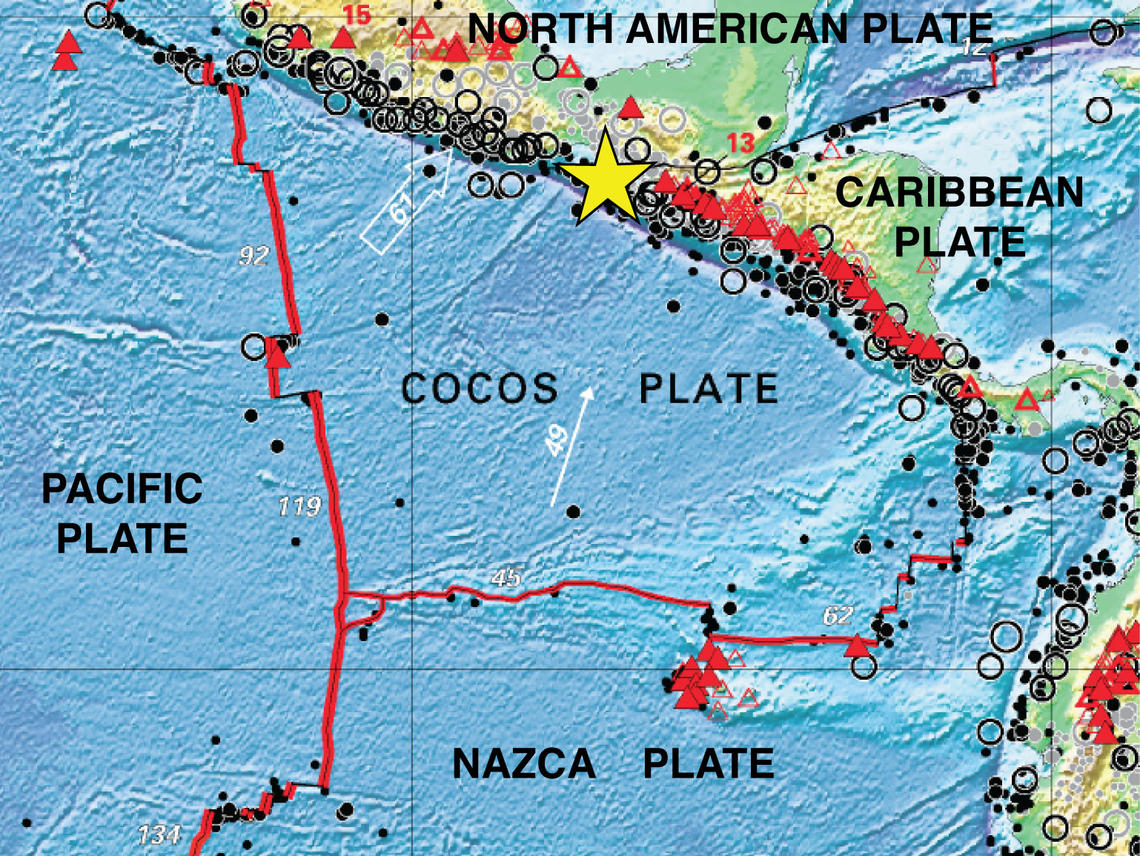
\includegraphics[width=0.85\textwidth]{./resources/Cocos}
    \caption{\cite{Cocos2006}}
  \end{figure}
\end{frame}

\begin{frame}
  \begin{figure}
    \centering
    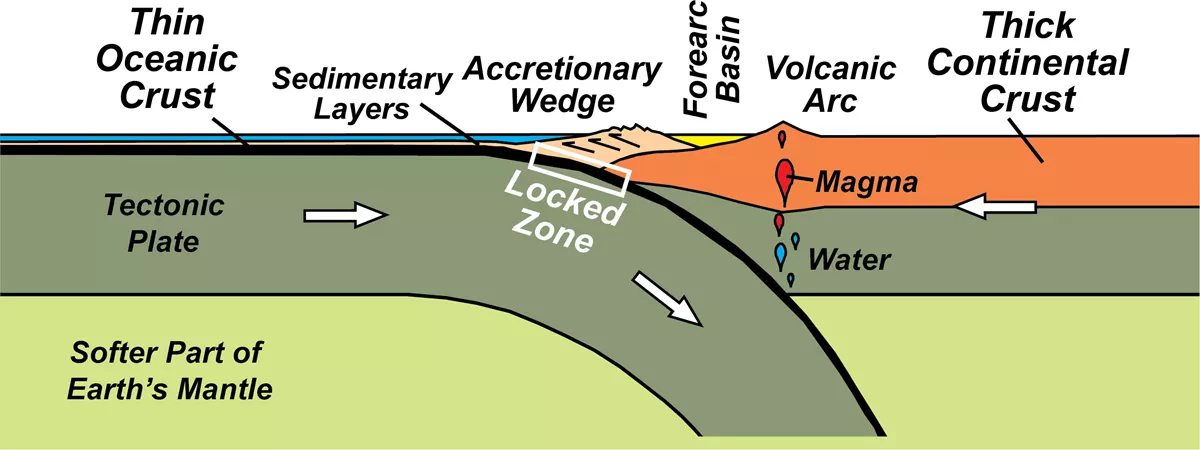
\includegraphics[width=\textwidth]{./resources/subduction_zone}
    \caption{\cite{Lillie2017}}
  \end{figure}
\end{frame}

\begin{frame}
  \frametitle{Goals}
  \begin{alertblock}{}
    \begin{center}
      {\large Understand the subduction zone from collected observations.}
    \end{center}
  \end{alertblock}
  \pause
  \begin{alertblock}{}
    \begin{center}
      {\large Do so while quantifying measurement uncertainties.}
    \end{center}
  \end{alertblock}
\end{frame}

\begin{frame}
  \frametitle{Table of Contents}
  \tableofcontents
\end{frame}

%%%%%%%%%%%%%%%%%%%%%%%%%%%%%%%%%%%%%%%%%%%%%%%%%%%%%%%%%%%%%%%%%%%%%%%%%%%%%%%
%%% Seismic Inversion Model Problem
%%%%%%%%%%%%%%%%%%%%%%%%%%%%%%%%%%%%%%%%%%%%%%%%%%%%%%%%%%%%%%%%%%%%%%%%%%%%%%%
\section{Seismic Inversion Model Problem}
\begin{frame}
  \frametitle{Model Assumptions}
  \begin{figure}
    \centering
    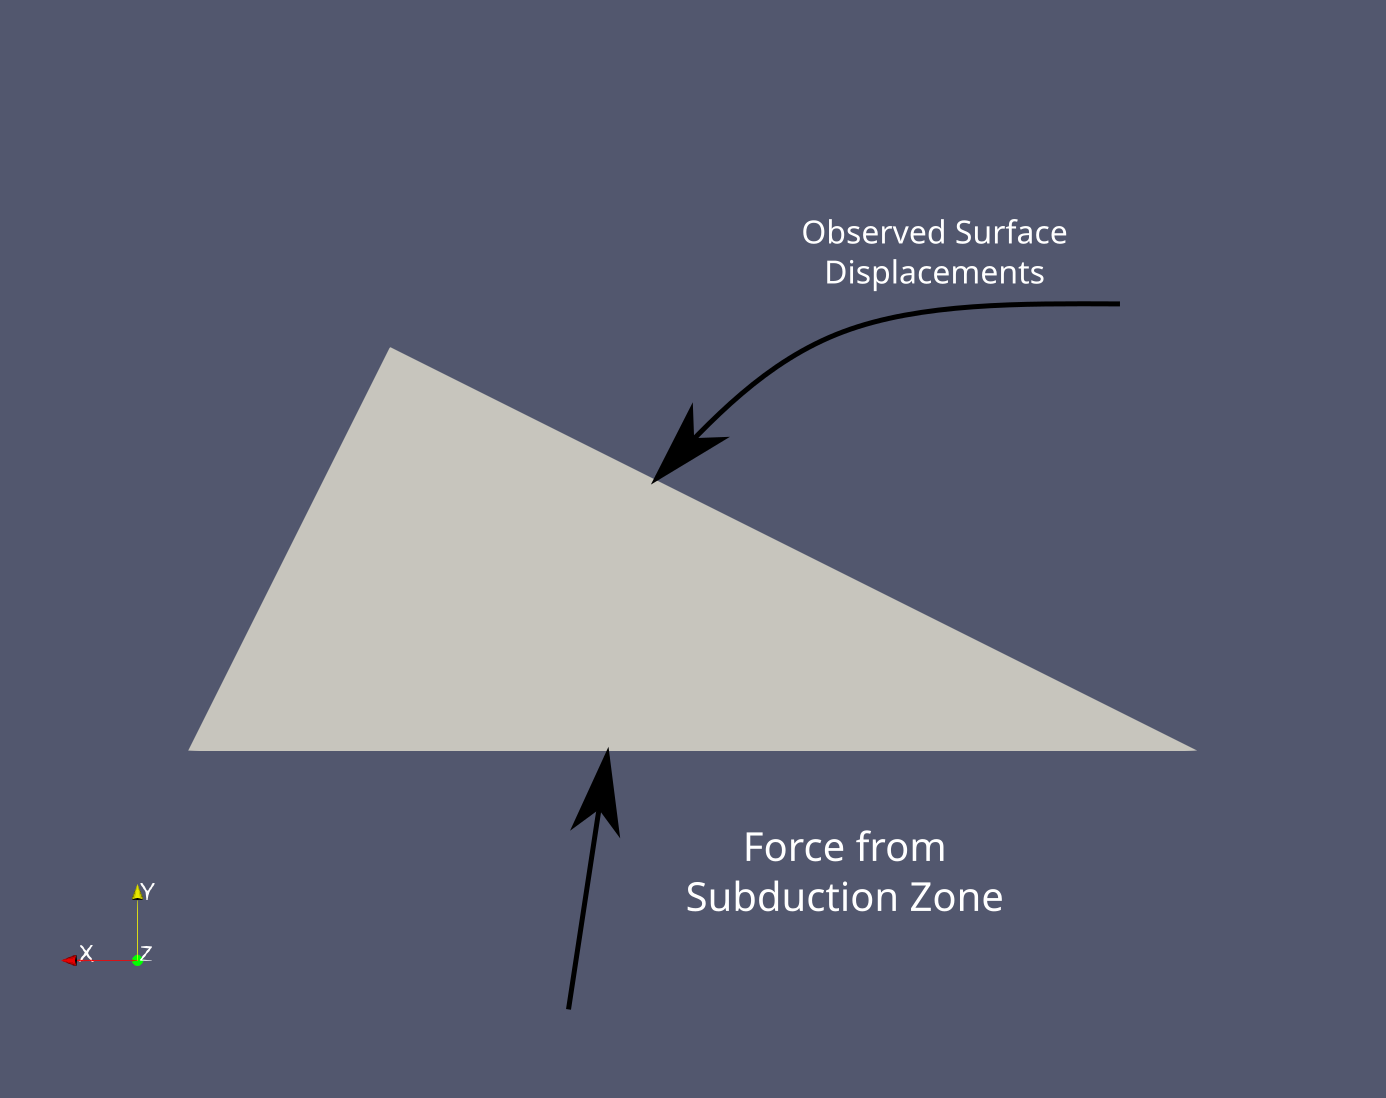
\includegraphics[width=0.55\textwidth]{./resources/triangle_paraview}
    %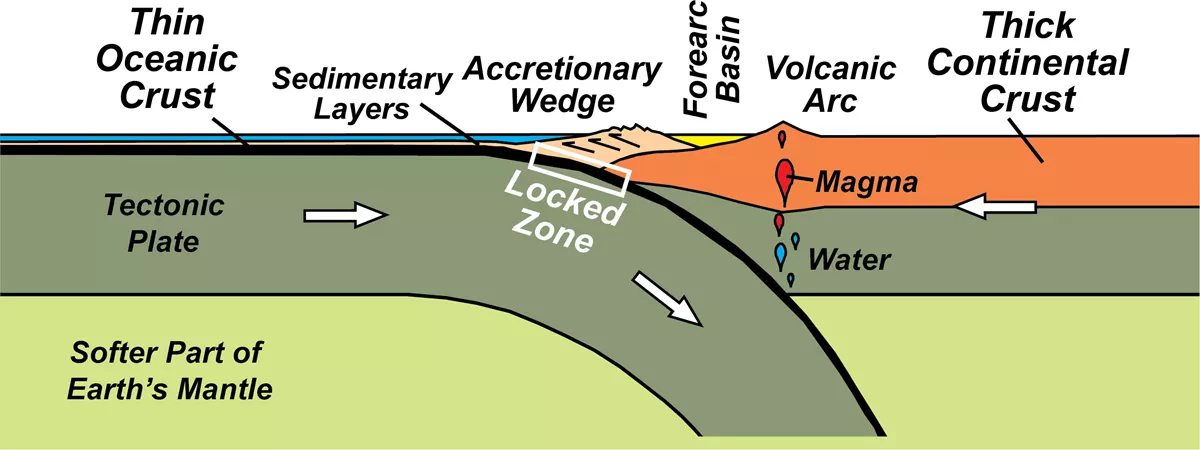
\includegraphics[width=\textwidth]{./resources/subduction_zone}
  \end{figure}
  For the sake of modeling convienience, assume:
  \begin{itemize}[<+->]
    \item \textbf{Governing PDE} (forward model): Linear elasticity
    \item \textbf{Uncertain parameter}: Displacement on fault plane
    \item \textbf{Inverse Problem}: Given measurements of surface deformation
      $\obs$ reconstruct fault plane displacement.
  \end{itemize}
\end{frame}
\begin{frame}
  \frametitle{Forward Model}
  \begin{equation}
    -\nabla \cdot \bs \sigma(\bs u) = \bs 0 \text{ in } \Omega,
  \end{equation}
  where:
  \begin{itemize}
    \item $\vec{\sigma}(\vec{u}) = \mathbb{C} \vec{\varepsilon}(\vec{u})$ with 
    \begin{itemize}
      \item $\mathbb{C}[\vec{\e}] = 2\mu \vec{\e} + \lambda \tr(\vec{\e})
        \mat{I}$ the fourth-order linear elasticity tensor:
      \item $\vec{\e}(\vec{u}) = \frac{1}{2} \left[ \grad \vec{u} + (\grad
        \vec{u})^\T \right]$ the strain tensor.
    \end{itemize}
  \item $\mu$ and $\lambda$ are known as the L\'{a}me constants.
  \end{itemize}
\end{frame}
\begin{frame}
  \frametitle{Forward Model}
  \begin{subequations}\label{eq:elast_strong}
    \begin{align}
      - \grad \left[ 
        \mu(\grad \vec{u} + (\grad \vec{u})^\T)
        + \lambda \div \vec{u} \mat{I}
      \right]
      &=
      \label{eq:elast_strong_a}
      \vec{0} \quad \text{in } \Omega, \\
      \label{eq:elast_strong_b}
      \vec{\sigma}(\vec{u}) \vec{n} 
      &= 
      \vec{0} \quad \text{on } \Gamma_t \\
      \label{eq:elast_strong_c}
      \vec{u} + \beta \vec{\sigma}(\vec{u}) \vec{n}
      &=
      \vec{h} \quad \text{on } \Gamma_s \\
      \label{eq:elast_strong_d}
      \vec{u} \vdot \vec{n} 
      &=
      0 \quad \text{on } \Gamma_b \\
      \label{eq:elast_strong_e}
      \delta \mat{T}(\vec{\sigma}(\vec{u})\vec{n}) + \mat{T}\vec{u}
      &=
      \vec{m} \quad \text{on } \Gamma_b
    \end{align}
  \end{subequations}
  \begin{itemize}[<+->]
    \item $\mat{T}$ is the tangential operator $\mat{T} \vec{u} = (\mat{I}
      - \vec{n} \otimes \vec{n}) \vec{u} = \vec{u} - (\vec{n}^\T \vec{u})
      \vec{n}$.
    \item The right hand side of \eqref{eq:elast_strong_e} is the displacement
      on the fault plane that is being inverted for.
    \item \eqref{eq:elast_strong_e} can be understood as a regularized Dirichlet
      condition.
  \end{itemize}
\end{frame}

\begin{frame}
  \frametitle{Forward Solution}
  \begin{figure}
    \centering
    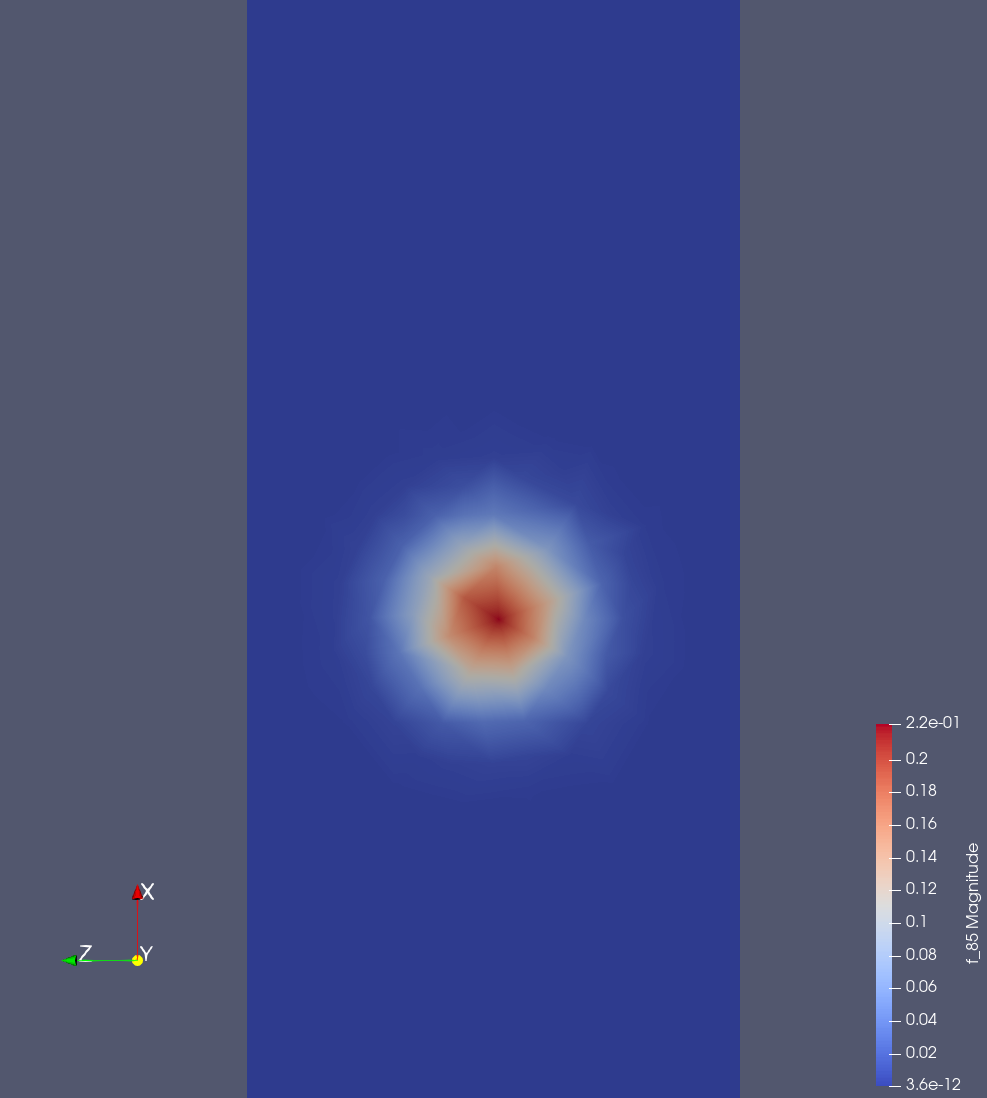
\includegraphics[width=0.49\textwidth]{./resources/fwd_bot}
    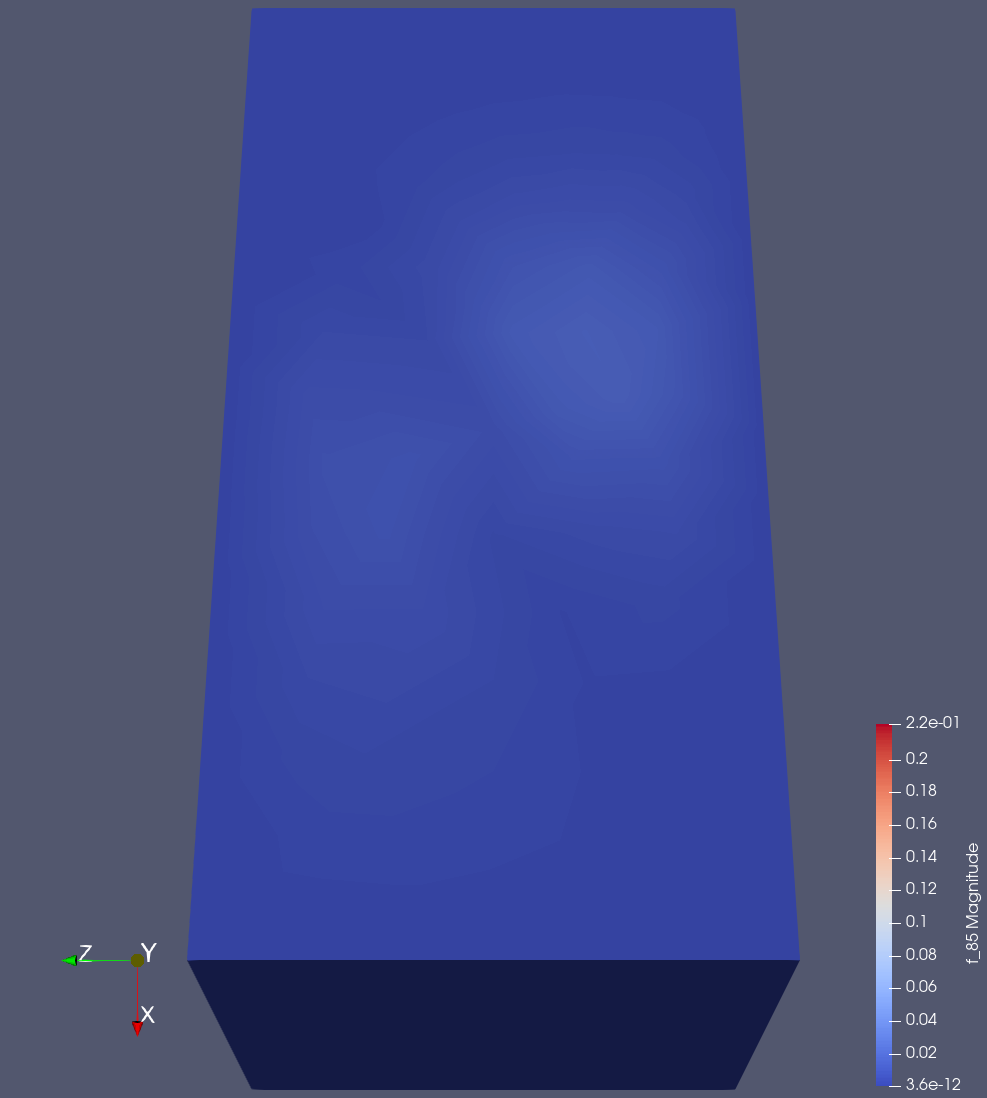
\includegraphics[width=0.49\textwidth]{./resources/fwd_top}
  \end{figure}
\end{frame}
\begin{frame}
  \frametitle{Forward Solution}
  \begin{figure}
    \centering
    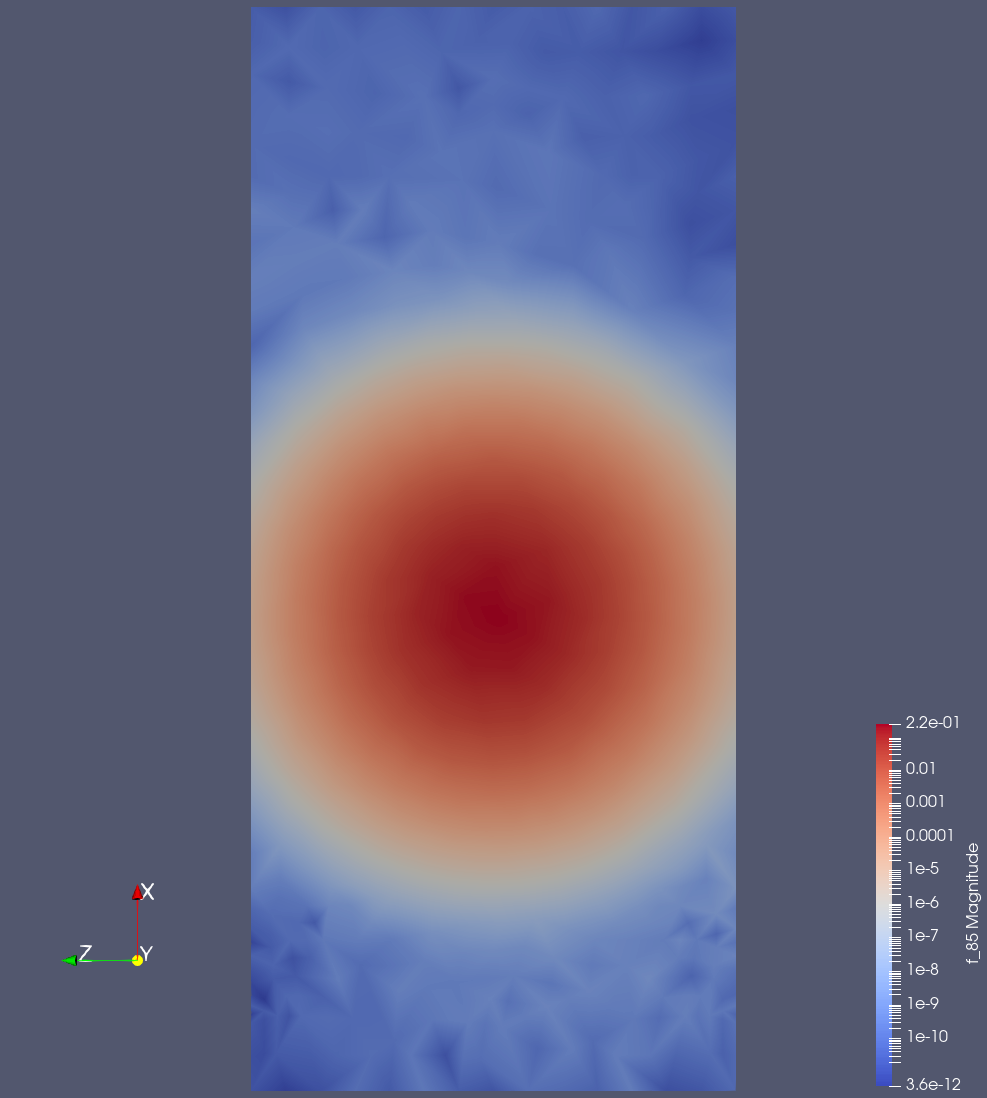
\includegraphics[width=0.49\textwidth]{./resources/fwd_bot_log}
    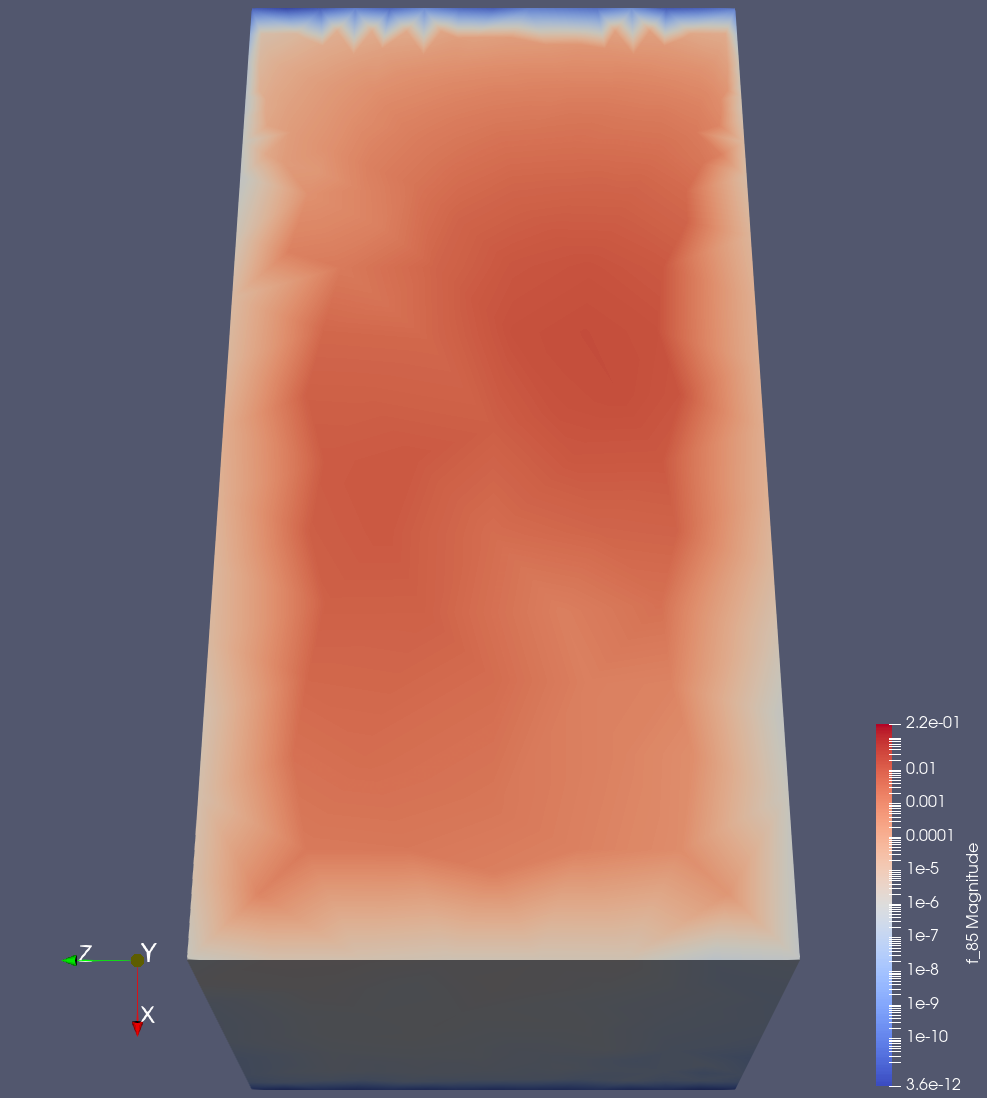
\includegraphics[width=0.49\textwidth]{./resources/fwd_top_log}
  \end{figure}
\end{frame}

\begin{frame}
  \frametitle{Weak Formulation}
  Define:
  \[
    \vec{V} \coloneqq
    \{ 
      \vec{u} \in H^1(\Omega)^3 
      : \vec{u} \vdot \vec{n} = 0 \text{ on } \Gamma_b
    \}
  \]
  Then the weak formulation of the forward model is given by:
  \begin{multline}
    \int_{\Gamma_s} \beta^{-1} (\vec{u} - \vec{h}) \vdot \vec{v} \dd{s}
    + \int_{\Gamma_b} \delta^{-1} (\mat{T} \vec{u} - \vec{m}) \vdot \vec{v}
    \dd{s} \\
    + \int_\Omega \vec{\e}(\vec{u}) : \mathbb{C}[\vec{\e}(\vec{v})] \dd{\vec{x}}
    = 0,
    \quad \forall v \in \vec{V}
  \end{multline}
\end{frame}

%%%%%%%%%%%%%%%%%%%%%%%%%%%%%%%%%%%%%%%%%%%%%%%%%%%%%%%%%%%%%%%%%%%%%%%%%%%%%%
%%% Bayesian Inversion Setting
%%%%%%%%%%%%%%%%%%%%%%%%%%%%%%%%%%%%%%%%%%%%%%%%%%%%%%%%%%%%%%%%%%%%%%%%%%%%%%%
\section{Infinite-Dimensional Inverse Problem Setting}
\begin{frame}
  \frametitle{The Deterministic Inverse Problem}
  To reconstruct the fault displacement we construct the PDE-constrained
  optimization problem:
  \[
    \mc{J}(\vec{m})
    = \min_\vec{m} \frac{1}{2} \| \mc{B}\vec{u}(\vec{m}) - \obs \|^2
    + \frac{1}{2} \| \mc{A}\vec{m} \|^2
  \]
  where $\vec{u}$ is given by the solution of the linear elasticity equation.
  \begin{itemize}
    \item $\vec{u}(\vec{m})$ is given by the forward model.
    \item $\mc{B}: (L^2(\Omega))^3 \to \R^N$ is an observation operator.
    \item $\obs \in \R^N$ where $N$ is the number of data points.
  \end{itemize}
  \pause
  If we let $\mc{S}$ be the forward model operator, i.e. $\vec{u} = \mc{S}
  \vec{m}$, and let\footnote{%
    In literature, called the {\em parameter-to-observable operator}.
  } $\mc{F} = \mc{B} \mc{S}$, then:
  \[
    \mc{J}(\vec{m})
    = \min_\vec{m} \frac{1}{2} \| \mc{F}\vec{m} - \obs \|^2
    + \frac{1}{2} \| \mc{A}\vec{m} \|^2
  \]
\end{frame}

\begin{frame}
  \frametitle{Bayes Inference in Infinite Dimensions}
\end{frame}


%%%%%%%%%%%%%%%%%%%%%%%%%%%%%%%%%%%%%%%%%%%%%%%%%%%%%%%%%%%%%%%%%%%%%%%%%%%%%%%
%%% Numerical Discretization and Considerations
%%%%%%%%%%%%%%%%%%%%%%%%%%%%%%%%%%%%%%%%%%%%%%%%%%%%%%%%%%%%%%%%%%%%%%%%%%%%%%%
\section{Numerical Discretization and Considerations}

%%%%%%%%%%%%%%%%%%%%%%%%%%%%%%%%%%%%%%%%%%%%%%%%%%%%%%%%%%%%%%%%%%%%%%%%%%%%%%%
%%% Results
%%%%%%%%%%%%%%%%%%%%%%%%%%%%%%%%%%%%%%%%%%%%%%%%%%%%%%%%%%%%%%%%%%%%%%%%%%%%%%%
\section{Results}

%%%%%%%%%%%%%%%%%%%%%%%%%%%%%%%%%%%%%%%%%%%%%%%%%%%%%%%%%%%%%%%%%%%%%%%%%%%%%%%
%%% Discussion and Future Work
%%%%%%%%%%%%%%%%%%%%%%%%%%%%%%%%%%%%%%%%%%%%%%%%%%%%%%%%%%%%%%%%%%%%%%%%%%%%%%%
\section{Discussion and Future Work}


%%%%%%%%%%%%%%%%%%%%%%%%%%%%%%%%%%%%%%%%%%%%%%%%%%%%%%%%%%%%%%%%%%%%%%%%%%%%%%%
%%% References
%%%%%%%%%%%%%%%%%%%%%%%%%%%%%%%%%%%%%%%%%%%%%%%%%%%%%%%%%%%%%%%%%%%%%%%%%%%%%%%
\section{References}
\begin{frame}[allowframebreaks]
  \frametitle{References}
  \bibliographystyle{amsalpha}
  \bibliography{citations.bib}
\end{frame}

\end{document}
